%%%
%
% $Autor: Wings $
% $Datum: 2021-05-14 $
% $Pfad: ArduinoLEDRGB $
% $Dateiname: 
% $Version: 4620 $
%
% !TeX spellcheck = de_DE/GB
% !TeX program = pdflatex
% !BIB program = biber/bibtex
% !TeX encoding = utf8
%
%%%

%todo citations
%todo create tikz pictures
%todo create sketches /ino-files with the code
%todo test the code


%https://projecthub.arduino.cc/semsemharaz/interfacing-rgb-led-with-arduino-b59902

% Farben: https://rgbcolorcode.com/color/00FF00


\chapter{Built-in RGB-LED}\index{LED!Built-in RGB-LED}

Some Arduino boards have a RGB-LED on board which can use for the application. ARG-LED is at least thre LEDs in on.

\section{General Information}

An RGB LED is a type of \ac{led} that can emit different colors of light. RGB stands for red, green, and blue, which are the three primary colors of light. An RGB LED consists of three individual \ac{led}s inside a single package, each with its own color and pin. By varying the brightness of each \ac{led} using \ac{pwm} signals, an RGB LED can produce a wide range of colors by mixing the primary colors. An RGB LED is usually active-low, which means that setting the pin to LOW will turn the \ac{led} on, and setting the pin to HIGH will turn the \ac{led} off. \cite{Bernstein:2018,Hering:2021,Karvinen:2014}

%\Mynote{cite English books}

\section{Specific Sensor}

The onboard LED of the Arduino Nano 33 BLE Sense is a RGB-LED that consists of three individual \ac{led}s: red, green, and blue. Each \ac{led} is connected to a different pin on the board:

\begin{itemize}
    \item Pin 22 for red,
    \item Pin 23 for green, and 
    \item Pin 24 for blue.
\end{itemize} 



The RGB-LED can produce different colors by varying the brightness of each \ac{led} using \ac{pwm} signals. The RGB-LED is active-low, which means that setting the pin to \PYTHON{LOW} will turn the \ac{led} on, and setting the pin to \PYTHON{HIGH} will turn the \ac{led} off. This is different from the power LED and the built-in LED, which are both active-high. \cite{ArduinoNanoGetStarted:2024,Arduino:2023a,Arduino:2023}



\bigskip

\begin{center}    
    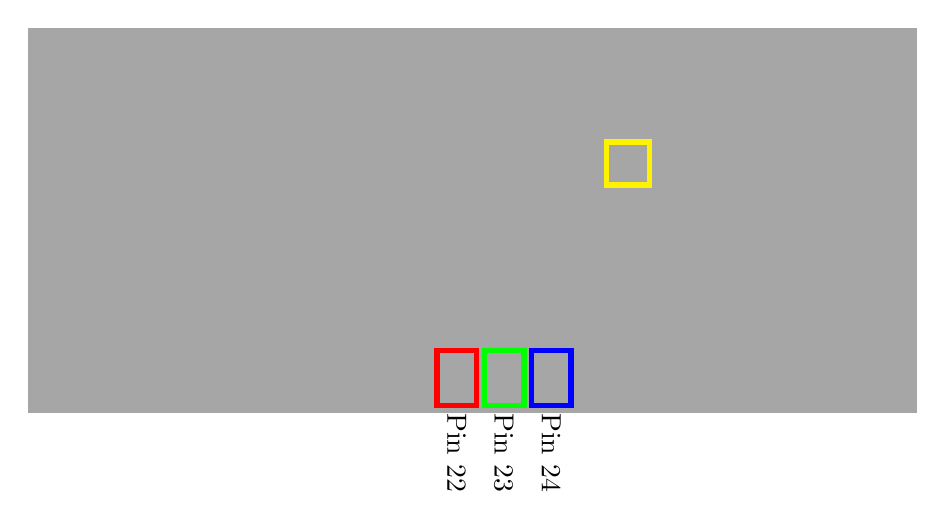
\begin{tikzpicture}
        %\node at (0,0) (Board) {\includegraphics{Arduino/Nano33BLE/Nano33BLESense}};
        
        \ArduinoNanoTikz;
        
        \fill[gray, opacity=0.7] (-11.2,-0.2) rectangle (0.1,4.7);
        
        \coordinate (A) at (-3.85,3.25);
        \coordinate (B) at (-3.3,2.7);    
        
        \coordinate (C) at (-4.8,0.6);
        \coordinate (D) at (-4.3,-0.1);    

        \coordinate (E) at (-5.4,0.6);
        \coordinate (F) at (-4.9,-0.1);    

        \coordinate (G) at (-6.0,0.6);
        \coordinate (H) at (-5.5,-0.1);    
        
        
        \begin{scope}
            \clip (A) rectangle (B);
            
            \ArduinoNanoTikz
            
            %\node at (0,0) (Board) {\includegraphics{Arduino/Nano33BLE/Nano33BLESense}};
            
        \end{scope}
        
        
        \draw[yellow,line width=2pt] (A)  rectangle (B);
        \draw[blue,line width=2pt] (C)  rectangle (D);
        \draw[green,line width=2pt] (E)  rectangle (F);
        \draw[red,line width=2pt] (G)  rectangle (H);
        
        \node[rotate=-90] (P25) at (-4.55, -0.7) {Pin 24};
        \node[rotate=-90] (P25) at (-5.15, -0.7) {Pin 23};
        \node[rotate=-90] (P25) at (-5.75, -0.7) {Pin 22};
    \end{tikzpicture}    
    
    \captionof{figure}{Arduino Nano 33 BLE Sense's RGB LED with Pin 22, Pin 23, and Pin 24}  
\end{center}

\bigskip



The brightness of the LED varies between 5000-6000 \ac{mcd} at a current of 20 mA. The color temperature is controllable and can be set in a range of 5000-6000 Kelvin. The LED should be stored and used between -40$^\circ$C and +85$^\circ$C.



\section{Specification}

\subsection{Pin Assignment}

The RGB LED occupies pins on the board internally. These pins are defined via variable names \PYTHON{LEDR}, \PYTHON{LEDG}, and \PYTHON{LEDB}. \cite{Arduino:2023a,Arduino:2023}

This must be observed when using the pins.



\begin{description}
    \item [Red LED:] LEDR = Pin 22\index{Pin!Pin 22,23,24}
    \item [Green LED:] LEDG = Pin 23
    \item [Blue LED:] LEDB = Pin 24
\end{description}


RGB LED is active-low and connected to pin 22, 23, and 24.

The RGB LED can be controlled programmatically by setting the pin to \PYTHON{LOW} or \PYTHON{HIGH}. 


%\Mynote{cite data sheet, power consumption?}

The pins 22, 23, and 24 must be defined as an output in the function \PYTHON{setup} by setting \PYTHON{pinMode (22, OUTPUT)}, \PYTHON{pinMode (23, OUTPUT)} and \PYTHON{pinMode (22, OUTPUT)}, otherwise the \ac{led} cannot be switched on.

\medskip 


The pins 22, 23, 24 can also be used otherwise. Then the \ac{led} is not in use.

\subsection{Power Comsumption}

The power comsumption has to be considered. It is the same value as for the power LED, see section~\ref{LEDPowerComsumption}. Here, a RGB-LED has 3 LEDs inside, therefore the poswer consumption must be consiederd for each color.




\section{Simple Code}


In the header file \FILE{RGBLED.h}, see code \ref{Nano:RGBLEDHeader}, are the declaration of the variables and the  functions. Variables are connected to pin 22, pin 23, and pin 24.\index{Pin!Pin 22}\index{Pin!Pin 23}\index{Pin!Pin 24} The pins are defined as output in the function \PYTHON{RGBLEDinit}. There are the following functions:

\begin{enumerate}
    \item \PYTHON{RGBLEDinit}: This funtion initializes the digital pin 22, pin 23, and pin 24 of the RGB-LED as output.
    \item \PYTHON{RGBLED\_Red}: This funtion switches the red part of the RGB-LED  on or off.
    \item \PYTHON{RGBLED\_Green}: This funtion switches the green part of the RGB-LED  on or off.
    \item \PYTHON{RGBLED\_Blue}: This funtion switches the blue part of the RGB-LED  on or off.
    \item \PYTHON{RGBLED\_Color}: This functions combines the colors.
\end{enumerate}

{
    \captionof{code}{Header file without comments for using the RGB-LED}\label{Nano:RGBLEDHeader}
    \ArduinoExternal{linerange={9-14,27-28,40-42}}{../../Code/Nano33BLESense/LEDs/RGBLED.h}
}

In the file \FILE{RGBLED.cpp}, see code \ref{Nano:RGBLEDCpp}, the functions are implemented.

{
    \captionof{code}{Code file without comments for using the RGB-LED}\label{Nano:RGBLEDCpp}
    \ArduinoExternal{linerange={12-15,28-34,46-51}}{../../Code/Nano33BLESense/LEDs/RGBLED.cpp}
}


\section{Tests}

\subsection{Simple Function Test}

The simplest test is the flashing of the \ac{led}s at 2 Hz, see sketch \ref{Nano:RGBEDTest}.

{
    \captionof{code}{Simple sketch to test the RGB LED}\label{Nano:RGBLEDTest}
    \ArduinoExternal{}{../../Code/Nano33BLESense/Test/TestLEDRGB.ino}
}


\subsection{Test all Functions}

\subsubsection{Different Colors}


\subsubsection{Colors}\index{LED!Colors}

A RGB LED is a device that can emit light of different colors by mixing the primary colors of red, green, and blue. The color of the light depends on the relative brightness of each \ac{led}, which can be controlled by \ac{pwm} signals. By varying the brightness of each \ac{led}, the RGB LED can produce a wide range of colors, such as yellow, cyan, magenta, white, and more. Some examples of the colors and their corresponding brightness values are:

\begin{description}
    \item [Red:] red = 255, green = 0, blue = 0
    \item [Green:] red = 0, green = 255, blue = 0
    \item [Blue:] red = 0, green = 0, blue = 255
    \item [Yellow:] red = 255, green = 255, blue = 0
    \item [Cyan:] red = 0, green = 255, blue = 255
    \item [Magenta:] red = 255, green = 0, blue = 255
    \item [White:] red = 255, green = 255, blue = 255
    \item [Black:] red = 0, green = 0, blue = 0
\end{description}

\medskip

The RGB LED can also create intermediate colors by using different brightness values for each \ac{led}. For example, to create

\begin{itemize}
    \item \textbf{orange}, one can use red = 255, green = 127, blue = 0. 
    \item To create \textbf{pink}, one can use red = 255, green = 192, blue = 203. 
    \item To create \textbf{purple}, one can use red = 128, green = 0, blue = 128. 
\end{itemize}


\bigskip

The sketch \ref{Nano:RGBLEDTestColors} tests different colors of the \ac{led}. The color of the \ac{led} changes every 1 second.

{
  \captionof{code}{value between 0 and 255  to write to the RGB LED}\label{Nano:RGBLEDTestColors}

  \ArduinoExternal{}{../../Code/Nano33BLESense/Test/TestLEDRGBColors.ino}
}



\subsubsection{Brightness of the RGB-LED}\index{LED!Brightness}

The RGB-LED can also create gradients of colors by changing the brightness values gradually over time. This can create a smooth transition from one color to another, such as from red to green to blue and back to red.

This sketch \ref{RGBLEDBrightness} will make the RGB-LED change colors smoothly by varying the brightness of each \ac{led} with different speeds. You can adjust the initial brightness values and the increment/decrement values to get different effects.


{
   \captionof{code}{Different brightness levels for the RGB-LED colors}\label{RGBLEDBrightness}
   \ArduinoExternal{}{../../Code/Nano33BLESense/Test/TestLEDRGBBrightness.ino}
}


\section{Simple Application}

In many applications, it is necessary to save power so that the \ac{led} is not switched on continuously. Nevertheless, feedback is required as to whether the system, e.g. a fire detector, is switched on and functional. In this case, the \ac{led} is switched on for 1 second at a defined time interval, in this case 30 seconds. This is implemented in the example \ref{Nano:TestRGBLEFApp}.

{
    \captionof{code}{A simple watch dog: A simple watchdog: the built-in RGB-LED is switched on for 1 second every 30 seconds.}\label{Nano:TestRGBLEDApp}
    \ArduinoExternal{}{../../Code/Nano33BLESense/Test/TestLEDRGBApplication.ino}
}



\section{Further Readings}

\begin{itemize}
  \item  Schanda, Janos: \textsl{Colorimetry: Understanding the CIE System}. Wiley, 2007. \cite{schanda:2007}
   \item Hiller, Gabrielle: \textsl{Color measurement - the CIE color space}. Datacolor, 2019. \cite{hiller:2019}
   \item Lukac, Rastislav and Plataniotis, Konstantinos N.: \textsl{Color Image Processing: Methods and Applications}. CTC Press, 2018. \cite{lukac:2018}
\end{itemize}



%%%%%%%%%%%%%%%%%%%%%%%%%%%%%%%%%%%%%%%%%%%%%%%%%%%%%%%%%


